%!TEX root = brainreader.tex

\section{Methods}

Our processing pipeline takes as input two pieces of data for each second:

\begin{itemize}
\item The top 100 guesses (based on fMRI data) - each guess has 15 frames
\item The log-likelihood (LLH) of each guess
\end{itemize}

We experimented with a variety of options for the 5 core steps of \emph{Weeding}, \emph{Forced Alignment}, \emph{Flow Calculation}, \emph{Pathfinding}, and \emph{Visualization} (see Figure \ref{fig:system}).

\begin{figure}
\centering
    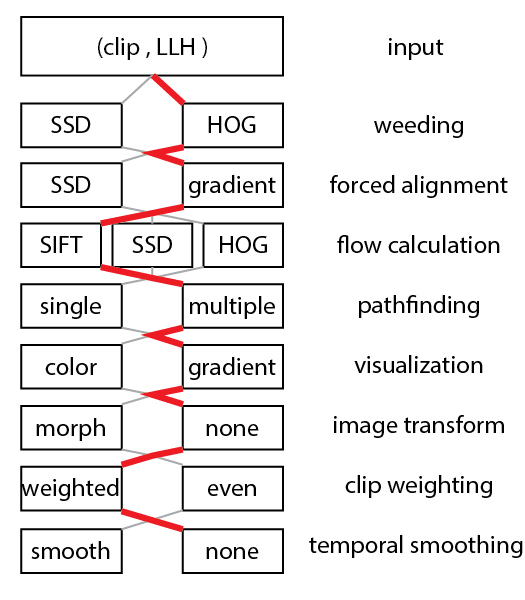
\includegraphics[width=1.0\columnwidth]{figures/system.png}
\caption{We experimented with a variety of options for the five core steps of Preprocessing, Forced Alignment, Flow Calculation, Pathfinding, and Visualization.  Highlighted in red is the most effective path.}
\label{fig:system}
\end{figure}

There are a few processes that we used for several steps in our pipeline, described here for later reference:

\emph{SSD} - Sum of Squared Differences (SSD) is a single number that represents a ``match'' score between two images.  It takes into account differences across the images' respective color channels, squaring and summing those differences to create one number indicating overall different-ness.

\emph{HOG} - Histogram of Oriented Gradients (HOG) descriptors focus on an image's edge data.  The descriptor has a variety of bins representing orientations and locations: images with similar HOG descriptors have similar edge orientations in similar spatial locations \cite{HOG}.

\emph{Gradient} - An image's gradient represents change in the image rather than absolute values.  Large changes in the image typically correspond to edges.

\subsection{Weeding}
While clips are already "weeded" in some sense by the fMRI data search over the video clip database, in order to make an effective visualization we first discard clips that are obviously very different from each other.  In deference to our already-ranked data, we search for clips that are best aligned to the top-ranked guess at each time step.

There are two processes for this: \emph{SSD} and \emph{HOG}.  Intuitively, SSD should be better for preserving color in images, since it takes color into account, while HOG should be better at preserving edges in images.  Therefore, we would expect that HOG-weeded guess clips would have better internal edge consistency.  This appears to be true to some degree (see Figure \ref{fig:weeding}): therefore we select HOG as our weeding tool of choice (in spite of SSD's obvious superiority in time efficiency).

\begin{figure}
\centering
    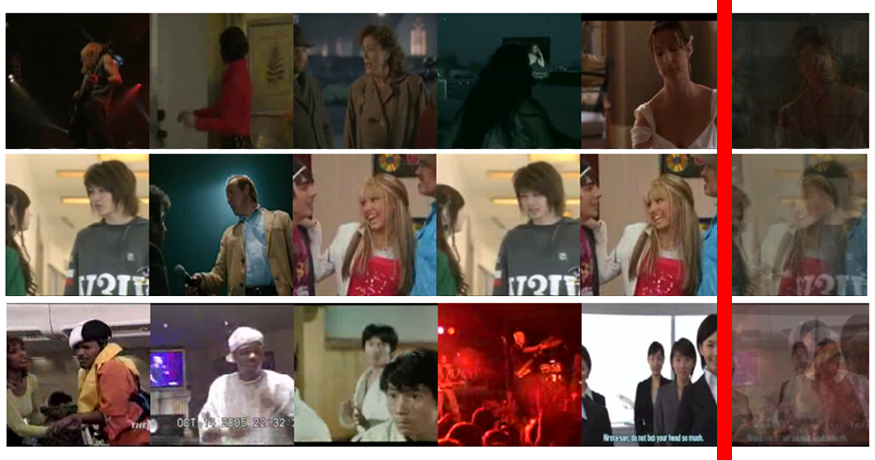
\includegraphics[width=1.0\columnwidth]{figures/preproc.png}
\caption{The top 5 guesses for one frame weeded based on SSD (top), HOG (middle), and LLH (bottom); and the sum of all five images (right).}
\label{fig:weeding}
\end{figure}

\subsection{Forced Alignment}
We forcibly align our guesses to each other: this makes the final visualization more pleasing, in addition to making flow calculations (discussed next) more meaningful.  The two forced alignment metrics we tested were \emph{SSD} and \emph{gradient}.

SSD-based alignment forcing encourages alignment of colors, while gradient-based alignment encourages alignment of edges.  Depending on the final visualization configuration, either may be desirable: if the visualization is going to be compiled in the color domain, color-based alignment may be best.  However, alignment in the gradient domain is more suited to visualization in the gradient domain (see Figure \ref{fig:align}).

\begin{figure}
\centering
    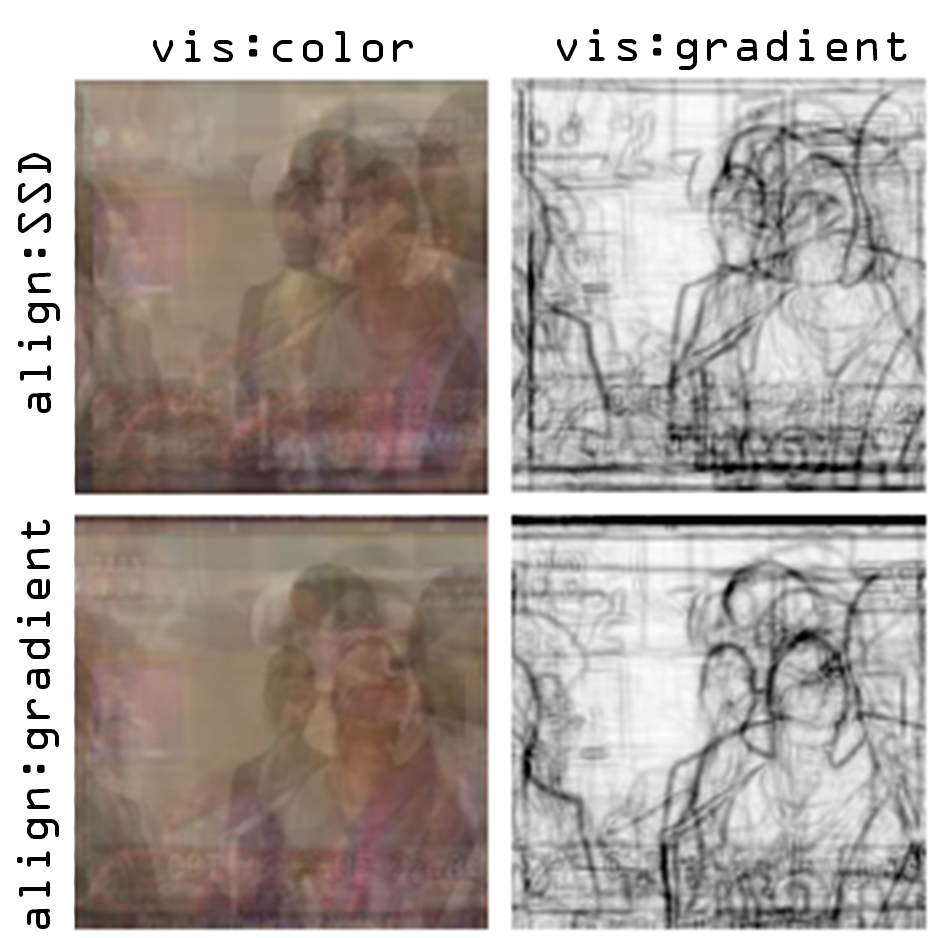
\includegraphics[width=1.0\columnwidth]{figures/align.png}
\caption{SSD-based alignment and gradient-based alignment lend themselves to different visualization techniques.  Here we show all possibilities of alignment technique x visualization technique: note that the lines match up best in the gradient domain when alignment is done there, and colors match up best when SSD is the alignment technique.}
\label{fig:align}
\end{figure}

For our final videos, we selected to use gradient-based alignment: visualizing our output in the gradient domain is more "true" to the fMRI data, which only accounts for shape and ignores color, and gradient-based alignment lends itself to gradient-based visualization.

\subsection{Flow Calculation}
We elected to reduce the number of clips shown in the final visualization from 100 to a much smaller number, which allows us some additional flexibility in stringing the clips together.  Instead of needing to create transitions from every clip from one time step into every clip from the next time step, we are able to take one or a few clips from the 100 best guesses and create a smooth path through those clips.

But what makes a ``smooth'' path?  Ideally, a smooth path is one where the last frame of one clip lines up with the first frame of the following clip: various techniques have been tried to determine the "difference" between two images.  \emph{SIFT flow} \cite{SIFTflow} finds SIFT keypoints in two images and estimates the ``flow'' of these keypoints between the two images.  This type of matching rewards scenes that are semantically, though perhaps not compositionally, similar: e.g., two images of streets would likely have low SIFT flow, while an image with a street at the bottom and an image with a river at the bottom would likely have high SIFT flow.  We had high hopes for this technique, however our dataset (only 100 guess clips per timestamp) did not enable us to find a visually smooth path using SIFT flow.

A second technique for path smoothness is \emph{SSD}.  Used in this part of the pipeline, SSD will ideally minimize jumps in color and composition between adjacent time steps, making clips flow smoothly into each other.

The final flow calculation we implemented was \emph{HOG}-based flow.  This again focuses on edge orientation and location, and lends itself to visualization consistency in the gradient domain.

We compare the various flow calculation techniques in Figure \ref{fig:flows}.

\begin{figure}
\centering
    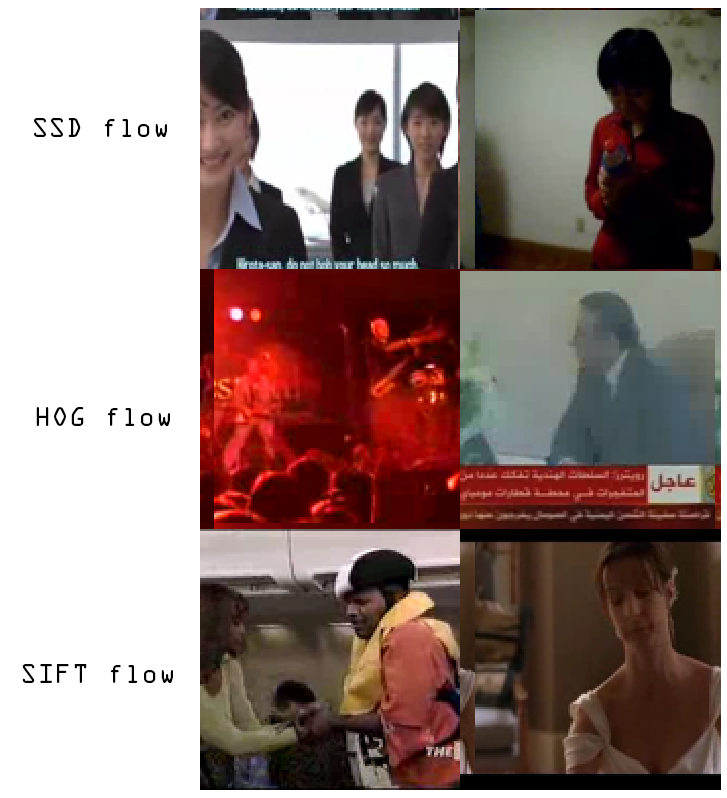
\includegraphics[width=1.0\columnwidth]{figures/lowflowstitled.png}
\caption{Various techniques can be used to calculate the ``difference'' between two images (in our case, the last frame of one clip and the first frame of the following clip).  We implemented SSD (focus on colors), HOG (focus on edges), and SIFT (focus on semantics).}
\label{fig:flows}
\end{figure}


\subsection{Pathfinding}
\natalia{write me}

\subsection{Visualization}
\natalia{write me}

\subsubsection{Gradient Domain}
\natalia{write me}

\subsubsection{Smoothing}
\natalia{write me}

\subsubsection{Overlay}
\natalia{write me}